%!TEX ROOT=ctutest.tex

%% Na obrazku lze videt xx obrazek ukazuje
%% trpny rod

\chapter{Softwarová implementace}

\section{Celkové chování systému}

\subsection{Komunikační protokol}
    Pro účely aplikace byl navržen komunikační protokol sloužící k rozlišení funkcionality jednotlivých paketů, přehlednou práci s přijatými nebo odesílanými daty a hlavně velmi dobrou budoucí rozšířitelnost celého systému.\\
    Každý radiopaket má pevně danou dvoubajtovou hlavičku, jež obsahuje  parametr \textit{CMD} determinující význam paketu a parametr \textit{sessionId}, který si lze představit podobně jako IP adresu, tedy specifikuje, komu je paket určen.\\
    Komunikační protokol je specifikovaný na straně brány v souboru \textit{radio\_packet.py} a na straně uzlu \textit{radio\_protocol.h}. 
    
    \todo{IMAGE: Doplnit obrázky}
    

\subsection{Zahájení komunikace – Join Process}
    Každá měřicí jednotka musí po svém restartu nejdříve zažádat o autorizaci u nejbližší brány. Tento proces probíhá prostřednictvím radiopaketu – JoinRequest, který je opakovaně odesílán, dokud brána neodpoví. Obsahem paketu je zejména unikátní čtyřbajtový identifikátor procesoru – \textit{uniqueId}, nulová jednobajtová adresa – \textit{sessionId} a časová známka sloužící pro pozdější časovou synchronizaci.\\
    Jakmile brána tento paket přijme je podle unikátní adresy zpracován a na jednotku je zpětně odeslán radiopaket JoinResponse s načtenou konfigurací z databáze a již konkrétní sessionId, která se dále využívá v průběhu celé další komunikace.
    
 \todo{TASK: Doplnit obrázky}
 
 \subsection{Nahrání konfigurace}
 \subsection{Konfigurace}


\section{Měřící jednotka (LoRa Node)}
\subsection{Použité softwarové nástroje}

%% opravdu to sem patri
    Software měřící jednotky byl napsán v programovacím jazyce C za použití vývojového prostředí Atollic TrueSTUDIO.\\
    Projekt byl založený na balíku dodaném firmou ST pro vývoj aplikací využívající LoRu – \textit{I-CUBE-LRWAN Expansion Package}.\\ 
    Z tohoto balíku byly využity zejména moduly pro obsluhu RF LoRa čipů od firmy Semtech SX1272/SX1276 (tedy PHY vrstva LoRaWAN protokolu), inicializace některých periferií a dodatečné nástroje jako třeba logování na konzoli.
    Implementace MAC vrstvy LoRaWAN protokolu využita nebyla z důvodů popsaných...
    \begin{figure} [h]
	    \centering
	    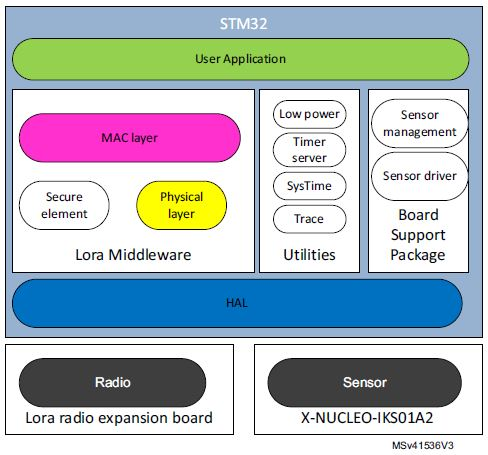
\includegraphics[ width = 0.8\textwidth]{SW_PART/Figs/st_loraextension.jpg}
        \caption {Hierarchie SW nástrojů dodaných firmou ST}
    \end{figure}  
    
    \todo{Misto, kde zduvodnim, proc nepouzivam LoRaWAN}
    
\subsection{Měřící jednotka – STATUS mód}
\subsection{Měřící jednotka – DEBUG mód}

   
%%Softwarový vývoj postavený na platformě ST může probíhat několika odlišnými způsoby. Lze využívat knihovnu obsahující pouze registry procesoru – CMSIS, kterou dodává samotný ARM nebo nízkoúrovňové knihovny LL (Low Level) či již komplexní knihovny HAL (Hardware Abstraction Layer), jejichž dodavatelem je ST. Pro vývoj měřící jednotky byl pou nakonec použita kombinace p  Obsluha komunikace MCU přes UART byla například naprogramována pouze pomocí CMSIS, obsluha AD převodníku pomocí LL a obsluha I2C pomocí HAL.
 %%
 
\section{Řídicí jednotka (LoRa Gateway)}
\subsection{Použité softwarové nástroje}
    Na Raspberry Pi byl v první řadě nainstalován operační systém Raspbian \cite{cite:3} ve verzi bez uživatelského rozhraní, který je založený na linuxovém Debianu a optimalizovaný pro Raspberry Pi. Pro samotný software řídící jednotky byl poté využit skriptovací programovací jazyk Python. Ten díky široké škále knihoven, které lze do projektu snadno importovat, usnadňuje vývojáři práci.\\
    Pro obsluhu GPIO pinů a periferií Raspberry jako SPI a UART byla využita knihovna \textit{wiringpi}.
    HTTP komunikaci s Node-RED serverem zabezpečovala knihovna \textit{requests} a TCP/IP komunikaci s TTN serverem knihovna \textit{socket}.
  
\subsection{Struktura aplikace – vícevláknový přístup}
    Z hlediska logické struktury byla aplikace rozdělena na hlavní vlákno a jednotlivá vlákna reprezentující připojené měřicí jednotky.\\
    Úkolem hlavního vlákna je neustále obsluhovat LoRa modul - přijímat a odesílat pakety. Tato obsluha musí probíhat neustále a nesmí být závislá na jiných okolnostech zdržujících její průběh, jako je komunikace s Node-RED servrem či zpracovávání přijatých informací.\\
    Ostatní vlákna zabezpečují úkoly jednotlivých měřicích jednotek. Zpracovávají přijatá naměřená data – radiopakety StatusInfo a odesílají je spolu s dalšími informacemi do Node-RED serveru.
   
    \todo{TASK:Vizualization of multithreading access}
    
    


\subsection{Řízení přístupu k rádiovému rozhraní}
    Jelikož řídicí jednotka umožňuje komunikovat s více měřicími jednotkami současně, je třeba brát ohled na využití rádiového LoRa modulu.\\
    V jednu chvíli se totiž může stát, že jedna jednotka bude odesílat informace o měření – radiopaket StatusInfo a druhé bude třeba z brány odeslat konfiguraci.
    
    Zprávy ze všech měřicích jednotek jsou přijaty v hlavním vlákně a to s nimi nakládá podle modelu producent-konzument. Přijatý paket rozešle do vláken všech komunikujících jednotek, které pak paket zpracují podle toho, jestli odpovídá jeho parametr \textit{sessionId}.\\
    Zprávy, které potřebuje brána odeslat daným měřicím jednotkám jsou nejprve vytvořeny v příslušném vláknu a přes společnou odesílací frontu jsou sdíleny s hlavním vláknem.
    
    Pro bránu je prioritní downlik, tedy odesílání zpráv. V hlavním cyklu se vždy kontroluje podmínka, že odesílací fronta je prázdná, pokud je přechází brána do RX (přijímacího) módu, ve kterém setrvá do vypršení timeoutu. Jakmile se tak stane a v odesílací frontě se objeví paket, je okamžitě odeslán a pokračuje se v cyklu. 
    \begin{figure} [h]
	    \centering
	    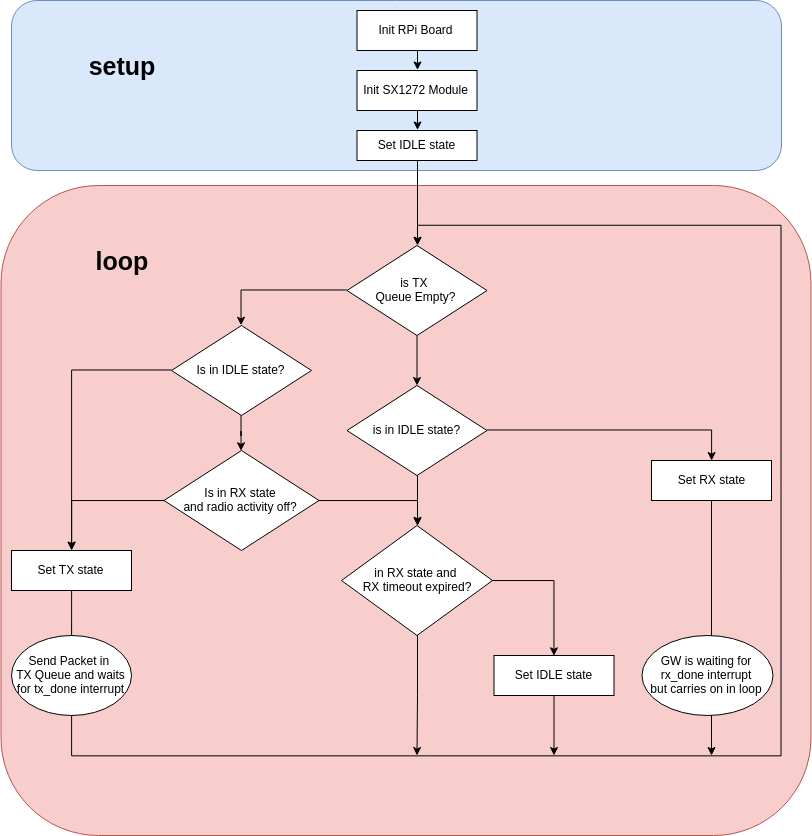
\includegraphics[ width = 0.9\textwidth]{SW_PART/Figs/GW_loop.png}
        \caption {Základní řídící smyčka hlavního vlákna brány}
    \end{figure}  
    
    
   
   
   
\section{Aplikační IoT server a databáze}
    Aplikační server a databáze jsou logicky odděleny od řídicí jednotky na Raspberry a mohou být umístěny kdekoliv na internetu, což umožňuje větší modularitu celého systému. Ve vytvořené demo aplikace byly ale všechny části umístěny na Rapberry Pi. Data jsou z řídicí jednotky nejprve umístěna do databáze. K vizualizaci slouží jednoduché uživatelské rozhraní, které data získává opětovnými SQL dotazy na databázi.
    
\subsection{Použité softwarové nástroje}
    Logika aplikačního serveru byla vytvořena na platformě Node-RED. Tento nástroj, vyvíjený společností IBM, je postavený na javascriptovém serveru Node.js a uživateli umožňuje pohodlně propojovat hardwarová zařízení, APIs (aplikační rozhraní) a online služby za pomocí flowchartového programování a to vše ve webovém rozhraní.\\ 
    Pro ukládání dat byla využita opensourcová databáze PostgreSQL. Jedná se o relační databázi, kde jednotlivé klíče (unikátní identifikátory typu GUID) udávají vztahy mezi tabulkami a záznamy v databázi.


\subsection{Komunikace s řídící jednotkou}
    Řídicí jednotka komunikuje se serverem prostřednictvím HTTP požadavků.\\
    Konfiguraci a informace o konkrétních uzlech získává brána prostřednictvím dotazu HTTP GET na url:\\ 
    \texttt{http://<Node-RED ip>:1880/app/config} či \\
    \texttt{http://<Node-RED ip>:1880/app/node\_params},\\
    kde v hlavičce dotazu specifikuje identifikační číslo daného uzlu. Jako odpověď přichází záznamy z databáze ve formátu JSON. IP adresa serveru se liší podle toho, kde je server umístěn, port je standardní – 1880.\\
    Pokud měřící jednotka pracuje ve STATUS módu, jsou do aplikačního serveru posílána data z měření, čehož lze docílit dvěma různými způsoby. Data lze odesílat na aplikační vrstvě osi-iso modelu pomocí HTTP POST dotazu na url:\\
    \texttt{http://<Node-RED ip>:1880/app/statusinfo}, \\
    kde se data společně s identifikačním číslem uzlu nacházejí v těle dotazu, nebo prostřednictvím transportní vrstvy pomocí UDP paketů na speciální port 8888.
    
    \todo{TASK: Vlozit tabulku s popisem url}
    
\subsection{Komunikace s aplikacemi třetích stran – REST API}
    Krom řídící jednotky je server připraven poskytovat data i aplikacím třetích stran, k čemuž slouží rozhraní vybudované na základě REST-JSON. S tímto rozhraním pak může komunikovat jakákoli další klientská aplikace, tedy například webový interface, který data získává pomocí javascriptu, nebo další připojený systém, což umožňuje koncovému uživateli velikou flexibilitu a rozšiřuje možnosti využití systému. 
    Data lze získat přes HTTP GET dotaz na stejné url jako v případě vkládání dat a pro přesnější výsledky je v rozhraní systému umožněno SQL-like dotazování použitím základních SQL struktur.
    
    \todo{TASK: Doplnit SQL-like dotazovaní}
  
    \todo{IMAGE: Doplnit o obrázek ze serveru}  
   
\subsection{Datový model}
    Pro účely aplikace byl vytvořen datový model, postavený na principech modelu relační databáze, který je znázorněn na obrázku.
    \begin{figure} [!h]
	    \centering
	    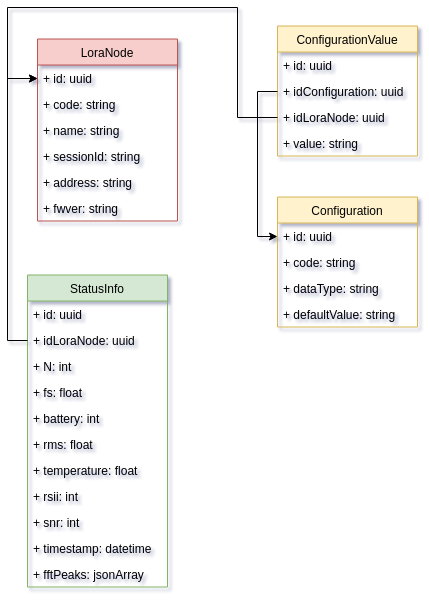
\includegraphics[ width = 0.8\textwidth]{SW_PART/Figs/data_model.png}
        \caption {UML diagram datového modelu aplikace}
    \end{figure} 
    
\subsection{Uživatelské rozhraní}
    V rámci serveru bylo vytvořeno také jednoduché uživatelské rozhraní, ve kterém jsou znázorněny časové změny monitorovaných veličin (teploty, RMS, stavu baterie, krest faktoru), nejvýznamnější píky ve frekvenčním spektru vibračního signálu a dodatečné informace o RSSI, SNR a časové známce   posledního přijatého paketu. Celé uživatelské rozhraní bylo vytvořeno za pomocí doplňku \textit{node-red-dashboard}.
    
    \todo{IMAGE: Pekny obrazek uzivatelskeho rozhrani}
    

    
    